 %package list
\documentclass{article}
\usepackage[top=3cm, bottom=3cm, outer=3cm, inner=3cm]{geometry}
\usepackage{multicol}
\UseRawInputEncoding
\usepackage{graphicx}
\usepackage{url}
%\usepackage{cite}
\usepackage{hyperref}
\usepackage{array}
%\usepackage{multicol}
\newcolumntype{x}[1]{>{\centering\arraybackslash\hspace{0pt}}p{#1}}
\usepackage{natbib}
\usepackage{pdfpages}
\usepackage{multirow}
\usepackage[normalem]{ulem}
\useunder{\uline}{\ul}{}
\usepackage{svg}
\usepackage{xcolor}
\usepackage{listings}
\lstdefinestyle{ascii-tree}{
    literate={├}{|}1 {─}{--}1 {└}{+}1
  }
\lstset{basicstyle=\ttfamily,
  showstringspaces=false,
  commentstyle=\color{red},
  keywordstyle=\color{blue}
}
%\usepackage{booktabs}
\usepackage{caption}
\usepackage{subcaption}
\usepackage{float}
\usepackage{array}

\newcolumntype{M}[1]{>{\centering\arraybackslash}m{#1}}
\newcolumntype{N}{@{}m{0pt}@{}}

%------------------------------ ÍTEMS --------------------------------

\newcommand{\itemEmail}{hchoquehuancaz@unsa.edu.pe}
\newcommand{\itemStudent}{Hernan Andy Choquehuanca Zapana}
\newcommand{\itemCourse}{Fundamentos de la Programacion II}
\newcommand{\itemCourseCode}{1701213}
\newcommand{\itemSemester}{II}
\newcommand{\itemUniversity}{Universidad Nacional de San Agustin de Arequipa}
\newcommand{\itemFaculty}{Facultad de Ingenieria de Produccion y Servicios}
\newcommand{\itemDepartment}{Departamento Academico de Ingenieria de Sistemas e Informatica}
\newcommand{\itemSchool}{Escuela Profesional de Ingenieria de Sistemas}
\newcommand{\itemAcademic}{2023 - B}
\newcommand{\itemInput}{Del 06 Diciembre 2023}
\newcommand{\itemOutput}{Al 11 Diciembre 2023}
\newcommand{\itemPracticeNumber}{12}
\newcommand{\itemTheme}{Definici\'on de Clases de Usuario}

%------------------------------  ------------------------------

\usepackage[english,spanish]{babel}
\usepackage[utf8]{inputenc}
\AtBeginDocument{\selectlanguage{Spanish}}
\renewcommand{\figurename}{Figura}
\renewcommand{\refname}{Referencias}
\renewcommand{\tablename}{Tabla} %esto no funciona cuando se usa babel
\AtBeginDocument{
	\renewcommand\tablename{Tabla}
}

\usepackage{fancyhdr}
\pagestyle{fancy}
\fancyhf{}
\setlength{\headheight}{30pt}
\renewcommand{\headrulewidth}{1pt}
\renewcommand{\footrulewidth}{1pt}
\fancyhead[L]{\raisebox{-0.2\height}{
\includegraphics[width=3cm]{img/logo_episunsa.png}}}
\fancyhead[C]{\fontsize{7}{7}\selectfont	\itemUniversity \\ \itemFaculty \\ \itemDepartment \\ \itemSchool \\ \textbf{\itemCourse}}
\fancyhead[R]{\raisebox{-0.2\height}{
\includegraphics[width=1.2cm]{img/logo_abet}}}
\fancyfoot[L]{Estudiante: Hernan Choquehuanca Zapana}
\fancyfoot[R]{\itemCourse}
\fancyfoot[C]{Página \thepage}

% para el codigo fuente
\usepackage{listings}
\usepackage{color, colortbl}
\definecolor{dkgreen}{rgb}{0,0.6,0}
\definecolor{gray}{rgb}{0.5,0.5,0.5}
\definecolor{mauve}{rgb}{0.58,0,0.82}
\definecolor{codebackground}{rgb}{0.95, 0.95, 0.92}
\definecolor{tablebackground}{rgb}{0.8, 0, 0}

\lstset{frame=tb,
	language=bash,
	aboveskip=3mm,
	belowskip=3mm,
	showstringspaces=false,
	columns=flexible,
	basicstyle={\small\ttfamily},
	numbers=none,
	numberstyle=\tiny\color{gray},
	keywordstyle=\color{blue},
	commentstyle=\color{dkgreen},
	stringstyle=\color{mauve},
	breaklines=true,
	breakatwhitespace=true,
	tabsize=3,
	backgroundcolor= \color{codebackground},
}

%------------------------------ INICIO DEL DOCUMENTO------------------------------

\begin{document}
	
	\vspace*{10px}
	
	\begin{center}	
		\fontsize{17}{17} \textbf{ Informe de Laboratorio \itemPracticeNumber}
	\end{center}
	\centerline{\textbf{\Large Tema: \itemTheme}}
	%\vspace*{0.5cm}	

	\begin{flushright}
		\begin{tabular}{|M{2.5cm}|N|}
			\hline 
			\rowcolor{tablebackground}
			\color{white} \textbf{Nota}  \\
			\hline 
			     \\[30pt]
			\hline 			
		\end{tabular}
	\end{flushright}	

	\begin{table}[H]
		\begin{tabular}{|x{4.7cm}|x{4.8cm}|x{4.8cm}|}
			\hline 
			\rowcolor{tablebackground}
			\color{white} \textbf{Estudiante} & \color{white}\textbf{Escuela}  & \color{white}\textbf{Asignatura}   \\
			\hline 
			{\itemStudent \par \itemEmail} & \itemSchool & {\itemCourse \par Semestre: \itemSemester \par Código: \itemCourseCode}     \\
			\hline 			
		\end{tabular}
	\end{table}		
	
	\begin{table}[H]
		\begin{tabular}{|x{4.7cm}|x{4.8cm}|x{4.8cm}|}
			\hline 
			\rowcolor{tablebackground}
			\color{white}\textbf{Laboratorio} & \color{white}\textbf{Tema}  & \color{white}\textbf{Duración}   \\
			\hline 
			\itemPracticeNumber & \itemTheme & 06 horas   \\
			\hline 
		\end{tabular}
	\end{table}
	
	\begin{table}[H]
		\begin{tabular}{|x{4.7cm}|x{4.8cm}|x{4.8cm}|}
			\hline 
			\rowcolor{tablebackground}
			\color{white}\textbf{Semestre académico} & \color{white}\textbf{Fecha de inicio}  & \color{white}\textbf{Fecha de entrega}   \\
			\hline 
			\itemAcademic & \itemInput &  \itemOutput  \\
			\hline 
		\end{tabular}
	\end{table}


%------------------------------ ACTIVIDADES (TAREA) ------------------------------

	\section{Tarea}
	\begin{itemize}		
        \item Puede reutilizar todo el código del laboratorio 11, pero ahora el objetivo es gestionar los ejércitos autogenerados.
        \item Al ejecutar el videojuego, el programa deberá dar las opciones:
        \item 1. Juego rápido (tal cual como en el laboratorio 11)
        Al acabar el juego mostrar las opciones de volver a jugar y de volver al menú principal. También se deberá tener la posibilidad de cancelar el juego actual en cualquier momento, permitiendo escoger entre empezar un juego totalmente nuevo o salir al menú principal.
        \item 2. Juego personalizado: permite gestionar ejércitos. Primero se generan los 2 ejércitos con sus respectivos soldados y se muestran sus datos.
        Luego se tendrá que escoger cuál de los 2 ejércitos se va a gestionar, después se mostrarán las siguientes opciones:
        \begin{itemize}
            \item 1) Crear Soldado: permitirá crear un nuevo soldado personalizado y añadir al final del ejército (recordar que límite es de 10 soldados por ejército)
            \item 2) Eliminar Soldado (no debe permitir un ejército vacío)
            \item 3) Clonar Soldado (crea una copia exacta del soldado) y se añade al final del ejército (recordar que límite es de 10 soldados por ejército)
            \item 4) Modificar Soldado (con submenú para cambiar alguno de los atributos nivelAtaque, nivelDefensa, vidaActual)
            \item 5) Comparar Soldados (verifica si atributos: nombre, nivelAtaque, nivelDefensa, vidaActual y vive son iguales)
            \item 6) Intercambiar Soldados (intercambia 2 soldados en sus posiciones en la estructura de datos del ejército)
            \item 7) Ver soldado (Búsqueda por nombre)
            \item 8) Ver ejército
            \item 9) Sumar niveles (usando Method-Call Chaining), calcular las sumatorias de nivelVida, nivelAtaque, nivelDefensa, velocidad de todos los soldados de un ejército
            1. Por ejemplo, si ejército tendría 3 soldados:
            2. s=s1.sumar(s2).sumar(s3);
            3. s es un objeto Soldado nuevo que contendría las sumatorias de los 4 atributos indicados de los 3 soldados. Ningún soldado cambia sus valores
            \item 10) Jugar (se empezará el juego con los cambios realizados) y con las mismas opciones de la opción 1.
            \item 11) Volver (muestra el menú principal)
        \end{itemize}

        Después de escoger alguna de las opciones 1) a 9) se podrá volver a elegir uno de los ejércitos y se mostrarán las opciones 1) a 11)
        \item 3. Salir

	\end{itemize}
		
\section{Equipos, materiales y temas utilizados}
	\begin{itemize}
		\item Sistema Operativo Windows 11 Pro 22H2 64 bits.
		\item Visual Studio Code.
		\item Git 2.42.0.
		\item Cuenta en GitHub con el correo institucional.
        \item Editor LaTeX en línea Overleaf.
        \item Variables Simples
        \item Métodos.
        \item Métodos de Búsqueda y Ordenamiento.
        \item HashMap
        
        
	\end{itemize}
	
\section{URL de Repositorio Github}
	\begin{itemize}
		\item URL del Repositorio GitHub para clonar o recuperar.
        \item \url{https://github.com/hernanchoquehuanca/fp2-23b.git}
		\item URL para el laboratorio 07 en el Repositorio GitHub.
		\item \url{https://github.com/hernanchoquehuanca/fp2-23b/tree/main/fase02/lab12}
	\end{itemize}
	
	\section{Trabajo del Laboratorio \itemPracticeNumber}
        
        
%-----------------------------------------------------------------------------------
%------------------------------------- ACTIVIDADES  --------------------------------
%-----------------------------------------------------------------------------------

% ACTIVIDADESSSS

%\subsection{Actividad 01}

\subsection{Clase Soldado.java}
\begin{lstlisting}[language=bash,caption={Commit \href{https://github.com/hernanchoquehuanca/fp2-23b/commit/9172d39d5d2f0483636ab831e8a91cc9c228dee4}{9172d39}: Se reutilizo las clases del laboratorio anterior}][H]
 $ git add .
 $ git commit -m "Se reutilizo las clases del laboratorio anterior"			
 $ git push -u origin main
\end{lstlisting}

\begin{itemize}	
    \item La clase \texttt{Soldado} se ha diseñado para representar a un soldado en un juego. Seguidamente, se describirán sus principales atributos y métodos:
    \begin{itemize}
        \item \texttt{private VideoJuego6 videoJuego6}: Una referencia al objeto de la clase \texttt{VideoJuego6}.
        \item \texttt{private String name}: El nombre del soldado.
        \item \texttt{private int row}: La fila en la que se encuentra el soldado.
        \item \texttt{private char column}: La columna en la que se encuentra el soldado.
        \item \texttt{private char team}: El equipo al que pertenece el soldado.
        \item \texttt{private int position}: La posición del soldado.
        \item \texttt{private int attackLevel}: El nivel de ataque del soldado.
        \item \texttt{private int levelDefense}: El nivel de defensa del soldado.
        \item \texttt{private int levelLife}: El nivel de vida original del soldado.
        \item \texttt{private int actualLife}: La vida actual del soldado.
        \item \texttt{private int speed}: La velocidad del soldado.
        \item \texttt{private String attitude}: La actitud del soldado.
        \item \texttt{private boolean lives}: Indica si el soldado está vivo o no.
    \end{itemize}
\end{itemize}
    \lstinputlisting[language=Java, firstline=2, lastline=15,firstnumber=2,numbers=left]{src/Soldado.java}

\begin{lstlisting}[language=bash,caption={Commit \href{https://github.com/hernanchoquehuanca/fp2-23b/commit/903d1c98abd3dedb3b72249a8f0d12acd297bfa2}{903d1c9}: Agregando los atributos solicitados a la clase Soldado}][H]
 $ git add .
 $ git commit -m "Agregando los atributos solicitados a la clase Soldado"			
 $ git push -u origin main
\end{lstlisting}

\begin{itemize}
    \item Se han implementado dos constructores para la clase \texttt{Soldado}:
    \begin{itemize}
        \item El primer constructor recibe todos los atributos como parámetros, inicializa los valores y asigna la referencia al objeto \texttt{VideoJuego6}.
    \end{itemize}
\end{itemize}
\lstinputlisting[language=Java, firstline=17, lastline=32,firstnumber=17,numbers=left]{src/Soldado.java}


\begin{itemize}
    \begin{itemize}
        \item El segundo constructor es una sobrecarga que asume que el soldado está vivo (\texttt{lives} establecido como \texttt{true}) y no recibe el parámetro \texttt{attitude}.
    \end{itemize}
\end{itemize}
\lstinputlisting[language=Java, firstline=34, lastline=47,firstnumber=34,numbers=left]{src/Soldado.java}

\begin{lstlisting}[language=bash,caption={Commit \href{https://github.com/hernanchoquehuanca/fp2-23b/commit/8afc11f2a3dd1fd16175506dc53913adde817dbe}{8afc11f}: Segundo avance del menu personalizado, se agrego un segundo constructor e implemento crear y eliminar soldados}][H]
 $ git add .
 $ git commit -m "Segundo avance del menu personalizado, se agrego un segundo constructor e implemento crear y eliminar soldados"			
 $ git push -u origin main
\end{lstlisting}

\newpage

\begin{itemize}
    \item Luego de ello también se implementaron los getters y setters para cada atributo de nuestra clase Soldado.
    \begin{itemize}
        \item Setters: 
    \end{itemize}
\end{itemize}
\lstinputlisting[language=Java, firstline=49, lastline=86,firstnumber=49,numbers=left]{src/Soldado.java}


\newpage %%%%%%%%%%%%%%%%%%%%%%

\begin{itemize}
    \begin{itemize}
        \item Getters: 
    \end{itemize}
\end{itemize}
\lstinputlisting[language=Java, firstline=88, lastline=128,firstnumber=88,numbers=left]{src/Soldado.java}

\begin{lstlisting}[language=bash,caption={Commit \href{https://github.com/hernanchoquehuanca/fp2-23b/commit/7c8c0c01d6e76ec195678846c285f0a2c8c58101}{7c8c0c0}: Se  completaron métodos que se utilizarán en la clase principal VideoJuego6.java}][H]
 $ git add .
 $ git commit -m "Completando los metodos de la clase soldado, ademas de adaptar el contructor principal"			
 $ git push -u origin main
\end{lstlisting}

\newpage %%%%%%%%%%%%%%%%%%%%%%

\begin{itemize}
    \item El método \texttt{toString()} se ha sobreescrito para proporcionar una representación en cadena de los atributos del soldado.
\end{itemize}

\lstinputlisting[language=Java, firstline=130, lastline=146,firstnumber=130,numbers=left]{src/Soldado.java}

\begin{itemize}
    \item Se han implementado varios métodos de acción para el soldado, como \texttt{attack()}, \texttt{defend()}, \texttt{advance()}, \texttt{back()}, \texttt{beAttacked()}, \texttt{flee()} y \texttt{die()}.
\end{itemize}
\lstinputlisting[language=Java, firstline=148, lastline=174,firstnumber=148,numbers=left]{src/Soldado.java}

  
\newpage %%%%%%%%%%%%%%%%%%%%%%

\subsection{Clase VideoJuego6.java}


\subsubsection{Método para la ejecución principal del juego}

\begin{itemize}
    \item El método tiene como nombre \textcolor{blue}{main()}.
    \item Recibe como parámetros un arreglo de cadenas \texttt{args}, aunque en este caso no se utiliza.
    \item Crea una instancia de la clase \texttt{VideoJuego6}.
    \item Llama al método \textcolor{blue}{createArmy()} para crear los ejércitos al inicio del juego.
    \item Llama al método \textcolor{blue}{mainInterfaz()} para gestionar la interfaz principal del juego.
\end{itemize}
\lstinputlisting[language=Java, firstline=14, lastline=18,firstnumber=14,numbers=left]{src/VideoJuego6.java}


\subsubsection{Método para interactuar con la Interfaz Principal}
\begin{itemize}
    \item El método tiene como nombre \textcolor{blue}{mainInterfaz()}.
    \item Se recibirá un número del 1 al 3 y se seleccionará la forma de juego o pedirá ingresar un número válido.
\end{itemize}
\lstinputlisting[language=Java, firstline=19, lastline=34,firstnumber=19,numbers=left]{src/VideoJuego6.java}


\newpage

\subsubsection{Método para mostrar la interfaz de juego rápido}
\begin{itemize}
    \item El método tiene como nombre \textcolor{blue}{quickGame()}.
    \item Al iniciar esta pequeña interfaz, se muestra las acciones que se pueden realizar, las cuales se eligen escribiendo un número del 1 - 8 según se desee.
    \item Al terminar cada caso desde el 1 al 7, se vuelve a llamar al mismo método, esto lo vuelve iterativo.
    \item En el caso \textcolor{blue}{1}, se hace el llamado al método \textcolor{blue}{createArmy()}.
    \item En el caso \textcolor{blue}{2}, se hace el llamado al método \textcolor{blue}{showArmyData()}.
    \item En el caso \textcolor{blue}{3}, se hace el llamado al método \textcolor{blue}{showArmyTable()}.
    \item En el caso \textcolor{blue}{4}, se hace el llamado al método \textcolor{blue}{averageHealth()}.
    \item En el caso \textcolor{blue}{5}, se hace el llamado al método \textcolor{blue}{moreHealth()}.
    \item En el caso \textcolor{blue}{6}, se hace el llamado al método \textcolor{blue}{printArmyHealth}.
    \item En el caso \textcolor{blue}{7}, se hace el llamado al método \textcolor{blue}{armyWinnerHealth()}.
    \item En el caso \textcolor{blue}{8}, se muestra el mensaje \textcolor{violet}{Fin} ya que esta opción termina el programa.
    \item Y por último en caso de no ser ningún número anteriormente mencionado, se muestra un mensaje indicando que se debe seleccionar una opción válida, y se hace un llamado nuevamente a la función.
\end{itemize}
\lstinputlisting[language=Java, firstline=35, lastline=96,firstnumber=35,numbers=left]{src/VideoJuego6.java}


\subsubsection{Método para la creación de los ejército}
\begin{itemize}
    \item El método tiene como nombre \textcolor{blue}{createArmy()}.
    \item Primero se define el número de soldados que contendrá cada ejército, haciendo uso de \textcolor{blue}{Math.random}.
    \item Ahora se llama dos veces al método \textcolor{blue}{createArmyTeam} para realizar la creación de los dos ejércitos a partir de los tamaños ya establecidos anteriormente y además el argumento tipo char para el identificador de cada equipo.
\end{itemize}
\lstinputlisting[language=Java, firstline=98, lastline=104,firstnumber=98,numbers=left]{src/VideoJuego6.java}


\subsubsection{Método para la creación de ejércitos}
\begin{itemize}
    \item El método tiene como nombre \textcolor{blue}{createArmyTeam()}.
    \item Recibe como parámetros un entero que es el número de soldados del ejército, el HashMap de soldados a utilizar y un char que va al final del nombre de los soldados, esto último nos ayuda a identificarlos mejor.
    \item Utilizando un do while se crean posiciones aleatorias en el HashMap bidimensional, tomando como condición que dicha posición sea distinta de \textcolor{blue}{null}.
    \item Finalmente se crea el soldado asignando su posición como clave \textcolor{blue}{Integer}(el valor de la fila se guarda multiplicado por 10 sumándole el valor de la columna), el valor es el soldado y se almacena en cada HashMap y retorna el HashMap unidimensional con los soldados creados.
\end{itemize}
\lstinputlisting[language=Java, firstline=106, lastline=122,firstnumber=106,numbers=left]{src/VideoJuego6.java}


\subsubsection{Método para mostrar la tabla con el ejército}
\begin{itemize}
    \item El método tiene como nombre \textcolor{blue}{showArmyTable()}.
    \item El algoritmo utilizado para imprimir el tablero, ya fue explicado en los laboratorios anteriores, por ello se omite la explicación.
\end{itemize}
\lstinputlisting[language=Java, firstline=124, lastline=143,firstnumber=124,numbers=left]{src/VideoJuego6.java}

\begin{itemize}\begin{itemize}\item Un ejemplo de como se muestra en la siguiente imagen:
\end{itemize}\end{itemize}
\begin{figure}[H]
    \centering
    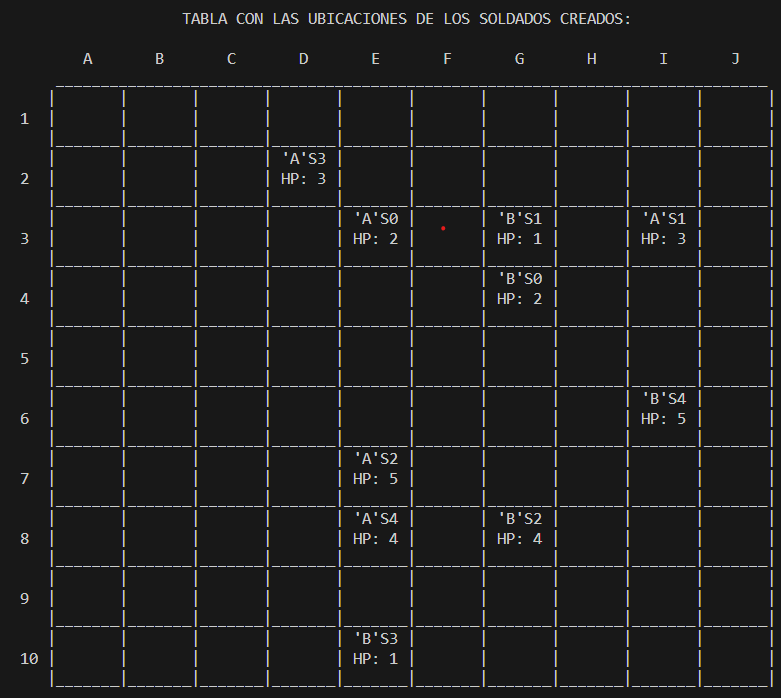
\includegraphics[width=1\textwidth,keepaspectratio]{img/showArmyTable.png}
    \caption{}
\end{figure}

\subsubsection{Método para mostrar los datos de los soldados de un ejército}
\begin{itemize}
    \item El método tiene como nombre \textcolor{blue}{showArmyData()}.
    \item Este usa un for each para recorrer el HashMap unidimensional de Soldado, y luego mostrar sus datos con el System.out.println, que a su vez este sigue el formato que se estableció en el método \textcolor{blue}{toString()} de la clase Soldado.java.
    \item La impresión en consola será la misma que la figura 1.
\end{itemize}
\lstinputlisting[language=Java, firstline=145, lastline=149,firstnumber=145,numbers=left]{src/VideoJuego6.java}


\subsubsection{Método para mostrar aquellos soldados con más vida de un ejército}
\begin{itemize}
    \item El método tiene como nombre \textcolor{blue}{moreHealt()}.
    \item Este recibe el HashMap con los soldados de un ejército, además de un char que indica el nombre del equipo.
    \item Primero recorre el HashMap unidimensional de soldados haciendo uso de un bucle for, de esta manera obtendrá el máximo de vida del ejército, el cual será almacenado en un entero maxHealth.
    \item Finalmente imprimirá aquellos soldados que tengan la vida igual a maxHealth, con un for y un if que controlará aquello.
    \item En la impresión se incluye el nombre del ejército antes de mostrar a los soldados.
\end{itemize}
\lstinputlisting[language=Java, firstline=151, lastline=162,firstnumber=151,numbers=left]{src/VideoJuego6.java}


\subsubsection{Método para hallar el promedio de vida en un ejército}
\begin{itemize}
    \item El método tiene como nombre \textcolor{blue}{averageHealth()}.
    \item De manera breve como el método, este retorna una división entre la suma de la vida del ejército, haciendo uso del método \textcolor{blue}{sumHealth()} y dividiendo entre el tamaño del ejército.
\end{itemize}
\lstinputlisting[language=Java, firstline=164, lastline=166,firstnumber=164,numbers=left]{src/VideoJuego6.java}


\subsubsection{Método para hallar la suma de vida en un ejército}
\begin{itemize}
    \item El método tiene como nombre \textcolor{blue}{sumHealth()}.
    \item Se utiliza un entero inicializado en 0 para mientras que se recorre el HashMap unidimensional de Soldado con un bucle for each, este entero (sum) va almacenando la vida de todos los soldados.
    \item Finalmente se retorna el entero \textcolor{blue}{sum}.
\end{itemize}
\lstinputlisting[language=Java, firstline=168, lastline=173,firstnumber=168,numbers=left]{src/VideoJuego6.java}


\subsubsection{Método de ordenamiento InsertionSort}
\begin{itemize}
    \item El método tiene como nombre \textcolor{blue}{insertionSort()}.
    \item El método tiene como finalidad ordenar el HashMap unidimensional de Soldado haciendo uso del algoritmo InsertionSort, tomando en cuenta la vida de los soldados que contiene cada soldado de dicho HashMap. Este algoritmo se extrajo de Geeksforgeeks y fue adaptado a este proyecto.
    \item \href{https://www.geeksforgeeks.org/insertion-sort/}{https://www.geeksforgeeks.org/insertion-sort/}
    \item CONCLUSIONES:
    \begin{itemize}
        \item El algoritmo recorre el HashMap desde el segundo soldado hasta el último, considerando cada vez al soldado como una "llave" y compara su salud con la de los soldados anteriores.
        \item Los soldaos son recorridos hacia la derecha en el HashMap hasta que se encuentren en la posición correcta según la vida del soldado "llave" actual. 
        \item El algoritmo de ordenamiento por inserción es más eficiente que el burbuja, pero a pesar de ello su complejidad sigue siendo de O($n^2$).
    \end{itemize}
\end{itemize}
\lstinputlisting[language=Java, firstline=174, lastline=189,firstnumber=174,numbers=left]{src/VideoJuego6.java}


\subsubsection{Método para imprimir los soldados de un ejército, ordenados según su vida}
\begin{itemize}
    \item El método tiene como nombre \textcolor{blue}{printArmyHealth()}.
    \item Este método recibirá un HashMap unidimensional de Soldado (previamente ordenado), lo recorrerá usando un bucle for y mostrará los soldados, teniendo en cuenta que primero se mostrarán los de mayor vida hasta los de menor.
\end{itemize}
\lstinputlisting[language=Java, firstline=190, lastline=194,firstnumber=190,numbers=left]{src/VideoJuego6.java}


\subsubsection{Método para seleccionar el equipo a personalizar}
\begin{itemize}
    \item El método tiene como nombre \textcolor{blue}{customGame()}.
    \item Se muestra los equipos disponibles a modificar, luego se recibe un entero que será la elección del usuario.
    \item Usando condicionales se elige el método adecuado para la elección.
    \item Se valida la entrada y luego se hace llamado al método \textcolor{blue}{customGameArmy()} enviando los respectivos argumentos.
\end{itemize}
\lstinputlisting[language=Java, firstline=196, lastline=208,firstnumber=196,numbers=left]{src/VideoJuego6.java}
\begin{itemize}\begin{itemize}\item Un ejemplo de como se muestra en la siguiente imagen:
\end{itemize}\end{itemize}
\begin{figure}[H]
    \centering
    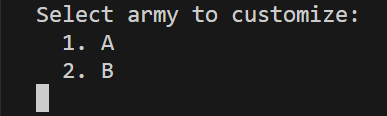
\includegraphics[width=0.5\textwidth,keepaspectratio]{img/12customGame.png}
    \caption{}
\end{figure}


\subsubsection{Método para mostrar la interfaz de juego personalizado}
\begin{itemize}
    \item El método tiene como nombre \textcolor{blue}{customGameArmy()}.
    \item Se muestra en pantalla las opciones y se recibe un entero valido que será la opción elegida por el usuario, para luego hacer un llamado al método correspondiente.
\end{itemize}
\lstinputlisting[language=Java, firstline=209, lastline=243,firstnumber=209,numbers=left]{src/VideoJuego6.java}

\newpage

\begin{itemize}\begin{itemize}\item Un ejemplo de como se muestra en la siguiente imagen:
\end{itemize}\end{itemize}
\begin{figure}[H]
    \centering
    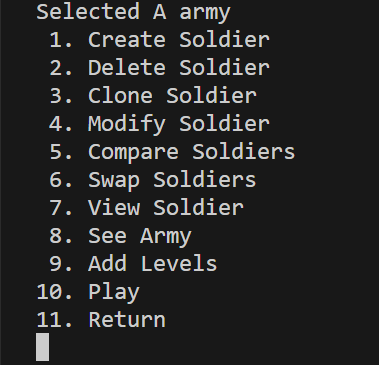
\includegraphics[width=0.5\textwidth,keepaspectratio]{img/12customGameArmy.png}
    \caption{}
\end{figure}


\subsubsection{Método para asignar los cambios realizados al ejercito elegido}
\begin{itemize}
    \item El método tiene como nombre \textcolor{blue}{assignModification()}.
    \item Se recibe el ejército personalizado y el char que contiene al equipo.
    \item Haciendo uso de una condicional se asigna al HashMap de clase del ejército correcto.
\end{itemize}
\lstinputlisting[language=Java, firstline=244, lastline=249,firstnumber=244,numbers=left]{src/VideoJuego6.java}

%\newpage

\subsubsection{Método para crear un soldado personalizado}
\begin{itemize}
    \item El método tiene como nombre \textcolor{blue}{createSoldier()}.
    \item En este método se recibe los datos del soldado a crear si el tamaño del ejército es menor a 10.
    \item Hace uso del método \textcolor{blue}{createPosition()} para los valores de la posición, en los demás casos los hace con el scanner y finalizada la recepción hace un llamado al segundo constructor.
\end{itemize}
\lstinputlisting[language=Java, firstline=250, lastline=273,firstnumber=250,numbers=left]{src/VideoJuego6.java}

\begin{itemize}\begin{itemize}\item Un ejemplo de como se muestra en la siguiente imagen:
\end{itemize}\end{itemize}
\begin{figure}[H]
    \centering
    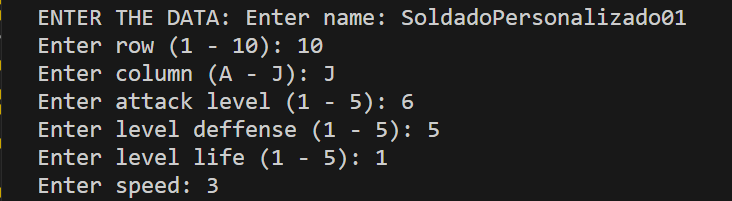
\includegraphics[width=0.8\textwidth,keepaspectratio]{img/12createSoldier.png}
    \caption{}
\end{figure}


\subsubsection{Método para crear una posición en el tablero}
\begin{itemize}
    \item El método tiene como nombre \textcolor{blue}{createPosition()}.
    \item El método recibe las coordenadas del soldado a crear y verifica que no esté ocupado, ya que en caso sea así este pedirá ingresar los datos nuevamente hasta que se ingrese un casillero vacío.
\end{itemize}
\lstinputlisting[language=Java, firstline=274, lastline=285,firstnumber=274,numbers=left]{src/VideoJuego6.java}


\subsubsection{Método para eliminar un soldado}
\begin{itemize}
    \item El método tiene como nombre \textcolor{blue}{deleteSoldier()}.
    \item Se muestra los soldados y luego se recibe el nombre del soldado a eliminar, se verifica que exista usando bucles y condicionales, en caso de que sí se eliminan del tablero principal y de l Hashmap de su equipo.
\end{itemize}
\lstinputlisting[language=Java, firstline=286, lastline=313,firstnumber=286,numbers=left]{src/VideoJuego6.java}

\begin{itemize}\begin{itemize}\item Un ejemplo de como se muestra en la siguiente imagen:
\end{itemize}\end{itemize}
\begin{figure}[H]
    \centering
    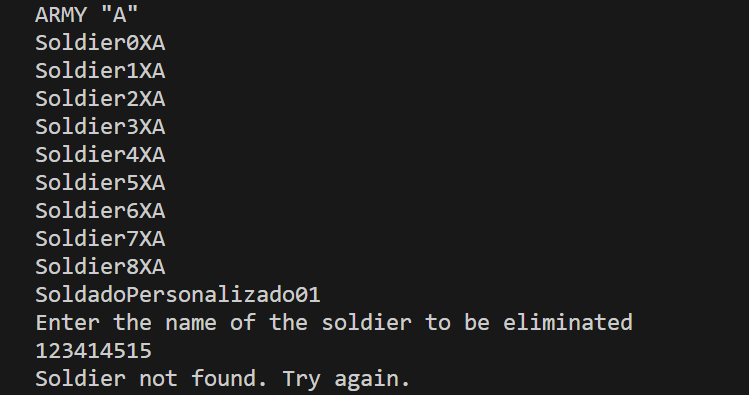
\includegraphics[width=0.6\textwidth,keepaspectratio]{img/12deleteSoldier.png}
    \caption{}
\end{figure}


\subsubsection{Método para clonar un soldado}
\begin{itemize}
    \item El método tiene como nombre \textcolor{blue}{cloneSoldier()}.
    \item Sigue la misma lógica de los métodos anteriores, solo que en este caso pide una posición para colocar el soldado clonado ya que no pueden haber 2 en la misma posición del tablero.
    \item En cuanto a lo demás realiza una copia de los atributos menos el del nombre ya que si se desearía utilizar en otro método no habría manera de saber a cual llamar.
\end{itemize}
\lstinputlisting[language=Java, firstline=314, lastline=353,firstnumber=314,numbers=left]{src/VideoJuego6.java}

\begin{itemize}\begin{itemize}\item Un ejemplo de como se muestra en la siguiente imagen:
\end{itemize}\end{itemize}
\begin{figure}[H]
    \centering
    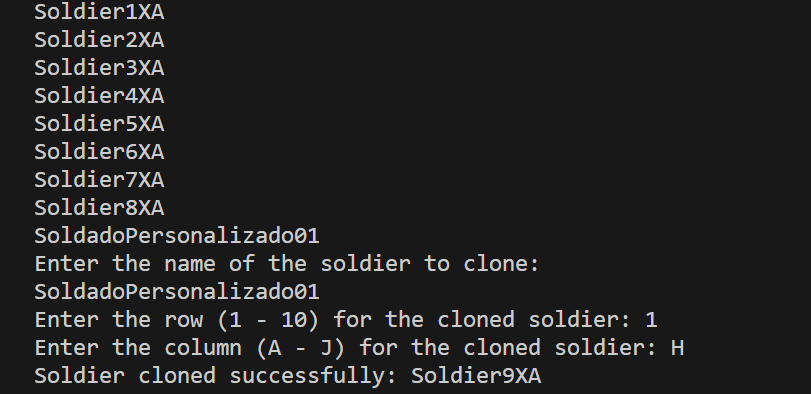
\includegraphics[width=0.65\textwidth,keepaspectratio]{img/12cloneSoldier.png}
    \caption{}
\end{figure}


\subsubsection{Método para modificar un soldado}
\begin{itemize}
    \item El método tiene como nombre \textcolor{blue}{modifySoldier()}.
    \item Primeramente se muestra el ejército y se solicita ingresar el nombre del soldado a modificar.
    \item Se verifica que exista y luego de ello se muestra las opciones a modificar, se recibe la elección y se usa un switch para cada opción.
    \item Por último solo se le asigna el nuevo valor recibido al soldado.
\end{itemize}
\lstinputlisting[language=Java, firstline=354, lastline=404,firstnumber=354,numbers=left]{src/VideoJuego6.java}

\begin{itemize}\begin{itemize}\item Un ejemplo de como se muestra en la siguiente imagen:
\end{itemize}\end{itemize}
\begin{figure}[H]
    \centering
    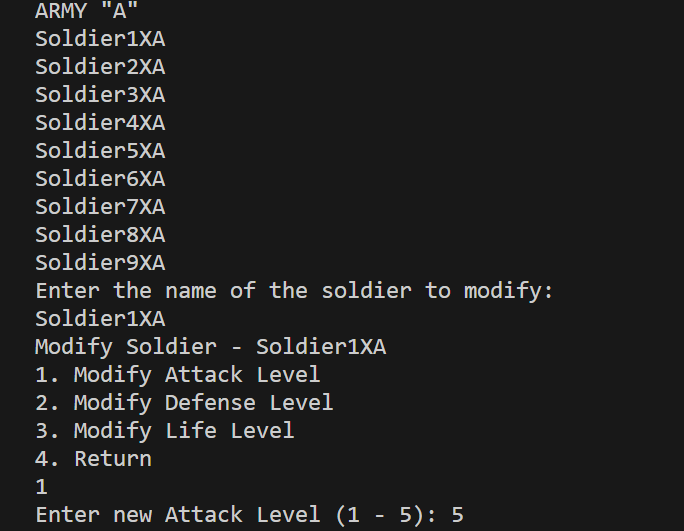
\includegraphics[width=0.65\textwidth,keepaspectratio]{img/12modifySoldier.png}
    \caption{}
\end{figure}

\newpage


\subsubsection{Método para comparar soldados}
\begin{itemize}
    \item El método tiene como nombre \textcolor{blue}{compareSoldiers()}.
    \item Pide los nombres de los dos soldados a comparar, para luego verificar que exista y posteriormente hacer uso del método \textcolor{blue}{compareSoldadoAttributes()} y con uso de condicionales mostrar si son idénticos o no.
\end{itemize}
\lstinputlisting[language=Java, firstline=405, lastline=428,firstnumber=405,numbers=left]{src/VideoJuego6.java}

\begin{itemize}\begin{itemize}\item Un ejemplo de como se muestra en la siguiente imagen:
\end{itemize}\end{itemize}
\begin{figure}[H]
    \centering
    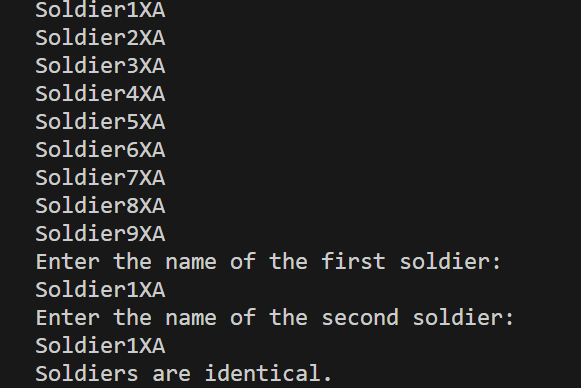
\includegraphics[width=0.65\textwidth,keepaspectratio]{img/12compareSoldiers.png}
    \caption{}
\end{figure}


\subsubsection{Método para buscar un soldado}
\begin{itemize}
    \item El método tiene como nombre \textcolor{blue}{findSoldado()}.
    \item Se envia el nombre del soldado como atributo junto a la estructura de datos que contiene su ejército, se usa un bucle for each para recorrer y retornar el soldado en caso exista.
\end{itemize}
\lstinputlisting[language=Java, firstline=429, lastline=434,firstnumber=429,numbers=left]{src/VideoJuego6.java}


\subsubsection{Método para comparar los atributos de un soldado}
\begin{itemize}
    \item El método tiene como nombre \textcolor{blue}{compareSoldadoAttributes()}.
    \item El método obtiene los atributos de ambos soldados y los compara dentro del mismo return.
\end{itemize}
\lstinputlisting[language=Java, firstline=435, lastline=441,firstnumber=435,numbers=left]{src/VideoJuego6.java}

\subsubsection{Método para intercambiar posiciones de 2 soldados}
\begin{itemize}
    \item El método tiene como nombre \textcolor{blue}{swapSoldiers()}.
    \item Muestra los soldados y luego recibe los nombres de los soldados a intercambiar verificando que existan.
    \item Posteriormente realiza las modificaciones tanto de sus atributos como en el tablero principal.
\end{itemize}
\lstinputlisting[language=Java, firstline=442, lastline=473,firstnumber=442,numbers=left]{src/VideoJuego6.java}

\begin{itemize}\begin{itemize}\item Un ejemplo de como se muestra en la siguiente imagen:
\end{itemize}\end{itemize}
\begin{figure}[H]
    \centering
    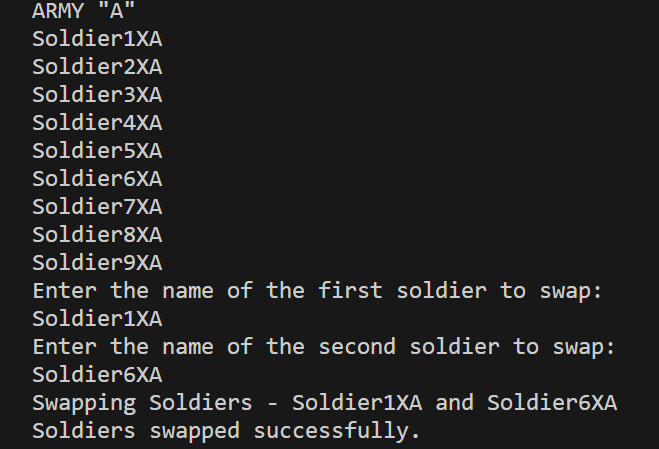
\includegraphics[width=0.65\textwidth,keepaspectratio]{img/12swapSoldiers.png}
    \caption{}
\end{figure}

\begin{lstlisting}[language=bash,caption={Commit \href{https://github.com/hernanchoquehuanca/fp2-23b/commit/c2bd05c15e26514a5164127762e717cb5792d561}{c2bd05c}: Septimo avance del metodo para jugabilidad de 2 jugadores, concluido hasta el lab11}][H]
 $ git add .
 $ git commit -m "Septimo avance del metodo para jugabilidad de 2 jugadores, concluido hasta el lab11"			
 $ git push -u origin main
\end{lstlisting}

\newpage

\subsubsection{Método para ver los datos de un soldado}
\begin{itemize}
    \item El método tiene como nombre \textcolor{blue}{viewSoldier()}.
    \item Muestra los soldados y solicita el nombre del soldado que se desea mostrar datos. Luego se busca el soldado y finalmente se muestra sus atributos.
\end{itemize}
\lstinputlisting[language=Java, firstline=474, lastline=496,firstnumber=474,numbers=left]{src/VideoJuego6.java}

\begin{itemize}\begin{itemize}\item Un ejemplo de como se muestra en la siguiente imagen:
\end{itemize}\end{itemize}
\begin{figure}[H]
    \centering
    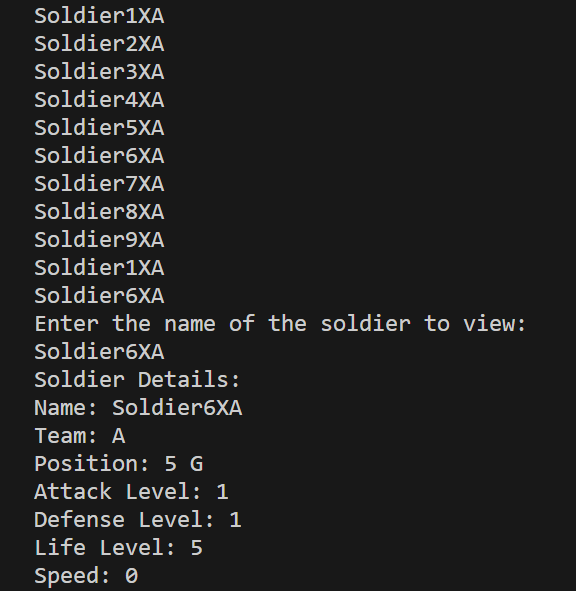
\includegraphics[width=0.45\textwidth,keepaspectratio]{img/12viewSoldier.png}
    \caption{}
\end{figure}


\subsubsection{Método para ver un ejército}
\begin{itemize}
    \item El método tiene como nombre \textcolor{blue}{seeArmy}.
    \item Sigue la misma lógica que el método anterior para ver soldados, de hecho podría reutilizarse para este método.
\end{itemize}
\lstinputlisting[language=Java, firstline=497, lastline=511,firstnumber=497,numbers=left]{src/VideoJuego6.java}


\subsubsection{Método para ver la sumatoria de niveles de un ejército}
\begin{itemize}
    \item El método tiene como nombre \textcolor{blue}{addLevels()}.
    \item El método usa un bucle for each para recorrer el ejército, luego va aumentando los valores de cada nivel de soldado para luego contenerlo en una variable entera y ser mostrada al final.
\end{itemize}
\lstinputlisting[language=Java, firstline=512, lastline=529,firstnumber=512,numbers=left]{src/VideoJuego6.java}

\begin{itemize}\begin{itemize}\item Un ejemplo de como se muestra en la siguiente imagen:
\end{itemize}\end{itemize}
\begin{figure}[H]
    \centering
    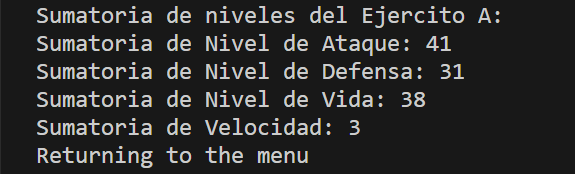
\includegraphics[width=0.6\textwidth,keepaspectratio]{img/12addLevels.png}
    \caption{}
\end{figure}


\subsubsection{Método para jugar ejército contra ejército}
\begin{itemize}
    \item El método tiene como nombre \textcolor{blue}{play()}.
    \item En este caso solo hace llamada al método \textcolor{blue}{gameInterfaz()}. que es la interfaz del juego 1v1.
\end{itemize}
\lstinputlisting[language=Java, firstline=530, lastline=532,firstnumber=530,numbers=left]{src/VideoJuego6.java}


\subsubsection{Método para mostrar al ejército ganador}
\begin{itemize}
    \item El método tiene como nombre \textcolor{blue}{amryWinner()}.
    \item Este método imprimirá al ejército ganador, usando como condición su tamaño.
    \item El método sólo será llamado cuando se verifique que uno de los dos ejércitos está vacío.
\end{itemize}
\lstinputlisting[language=Java, firstline=535, lastline=540,firstnumber=535,numbers=left]{src/VideoJuego6.java}


\subsubsection{Método para remover un soldado}
\begin{itemize}
    \item El método tiene como nombre \textcolor{blue}{removeSoldier()}.
    \item Obtiene el ejército al que pertenece y lo elimina tanto del HashMap de su ejército y del tablero de juego.
\end{itemize}
\lstinputlisting[language=Java, firstline=542, lastline=548,firstnumber=542,numbers=left]{src/VideoJuego6.java}


\subsubsection{Método para ejecutar la interfaz del juego}
\begin{itemize}
    \item El método tiene como nombre \textcolor{blue}{gameInterfaz()}.
    \item Se controla que el tamaño de los ejércitos no sea 0, de esta manera cuando lo sea se rompera el bucle while y se dará el nombre del ganador usando el método \textcolor{blue}{amryWinner()}.
\end{itemize}
\lstinputlisting[language=Java, firstline=549, lastline=566,firstnumber=549,numbers=left]{src/VideoJuego6.java}


\subsubsection{Método para la ejecución del turno del jugador}
\begin{itemize}
    \item El método tiene como nombre \textcolor{blue}{turn()}.
    \item Primero se comienza mostrando el tablero de juego. Luego se recibe las coordenadas del soldado a mover, para verificar se hace uso del método \textcolor{blue}{checkSoldier1()} y así llamar a \textcolor{blue}{turn2()}.
\end{itemize}
\lstinputlisting[language=Java, firstline=567, lastline=579,firstnumber=567,numbers=left]{src/VideoJuego6.java}

\begin{lstlisting}[language=bash,caption={Commit \href{https://github.com/hernanchoquehuanca/fp2-23b/commit/d8d54ce00cb19dbff9dc2f96c170e64cc9e1114a}{d8d54ce}: Se agregó los métodos para la jugabilidad de 2 (hasta lab10)}][H]
 $ git add .
 $ git commit -m "Sexto avance del metodo para jugabilidad de 2 jugadores, concluido hasta el lab10"	
 $ git push -u origin main
\end{lstlisting}

\subsubsection{Método para revisar que el soldado elegido sea válido}
\begin{itemize}
    \item El método tiene como nombre \textcolor{blue}{checkSoldier1()}.
    \item Este fue utilizado en el método anterior, verifica que las coordenadas estén dentro del tablero y pertenezca al equipo del cual es turno.
\end{itemize}
\lstinputlisting[language=Java, firstline=580, lastline=592,firstnumber=580,numbers=left]{src/VideoJuego6.java}


\subsubsection{Método para analizar la posición a mover}
\begin{itemize}
    \item El método tiene como nombre \textcolor{blue}{checkSoldier2()}.
    \item Esta es la segunda verificación ya que evalúa si se va a producir un movimiento a un casillero libre, hay un enemigo o aliado. Luego de eso regresa el entero según sea el caso.
\end{itemize}
\lstinputlisting[language=Java, firstline=593, lastline=601,firstnumber=593,numbers=left]{src/VideoJuego6.java}


\subsubsection{Método para ejecutar el movimiento elegido}
\begin{itemize}
    \item El método tiene como nombre \textcolor{blue}{turn2()}.
    \item Esté método recibe la coordenada a donde se desea mover el soldado que fue elegido previamente.
    \item Además de contener los posibles movimientos en caso sea válido, por ejemplo una pelea de soldados.
\end{itemize}
\lstinputlisting[language=Java, firstline=602, lastline=626,firstnumber=602,numbers=left]{src/VideoJuego6.java}


\subsubsection{Método para mover un soldado 1}
\begin{itemize}
    \item El método tiene como nombre \textcolor{blue}{moveSoldier()} y es sobrecargado.
    \item El método coloca el soldado en la posición previamente recibida y la remueve de su posición anterior.
\end{itemize}
\lstinputlisting[language=Java, firstline=627, lastline=630,firstnumber=627,numbers=left]{src/VideoJuego6.java}


\subsubsection{Método para mover un soldado 2}
\begin{itemize}
    \item El método tiene como nombre \textcolor{blue}{moveSoldier() y es sobrecargado}.
    \item Al contrario del método anterior este cuenta con parámetros distintos ya que incluye un soldado, pero realiza la misma función que el método anterior, pero este en caso de haber un soldado ganador de una pelea.
\end{itemize}
\lstinputlisting[language=Java, firstline=631, lastline=634,firstnumber=631,numbers=left]{src/VideoJuego6.java}


\subsubsection{Método para ejecutar la pelea de dos soldados}
\begin{itemize}
    \item El método tiene como nombre \textcolor{blue}{soldiersFight()}.
    \item Este método es uno de los más importantes ya que ejecuta la pelea entre dos soldados.
    \item Crea las probabilidades proporcionalmente a la suma de vida actual de ambos soldados.
    \item Muestra las probabilidades y luego elije de manera aleatoria con uso de Random de java.util, para finalmente mostrar al soldado ganador y llamar a los métodos necesarios que se encarguen de eliminar y mover los soldados según sea la situación.
\end{itemize}
\lstinputlisting[language=Java, firstline=635, lastline=659,firstnumber=635,numbers=left]{src/VideoJuego6.java}

\begin{lstlisting}[language=bash,caption={Commit \href{https://github.com/hernanchoquehuanca/fp2-23b/commit/b3523d07a3d8f518091cb0476244ef750107db75}{b3523d0}: Siendo este el último commit referente al trabajo del código (el último fue revisión)}][H]
 $ git add .
 $ git commit -m "Decimo avance del menu personalizado, se agrego el metodo para salir"			
 $ git push -u origin main
\end{lstlisting}

     

%----------------------------- DIAGRAMA DE CLASE UML -------------------------------

\newpage

\subsection{Diagrama de clase UML}
\begin{figure}[H]
    \centering
    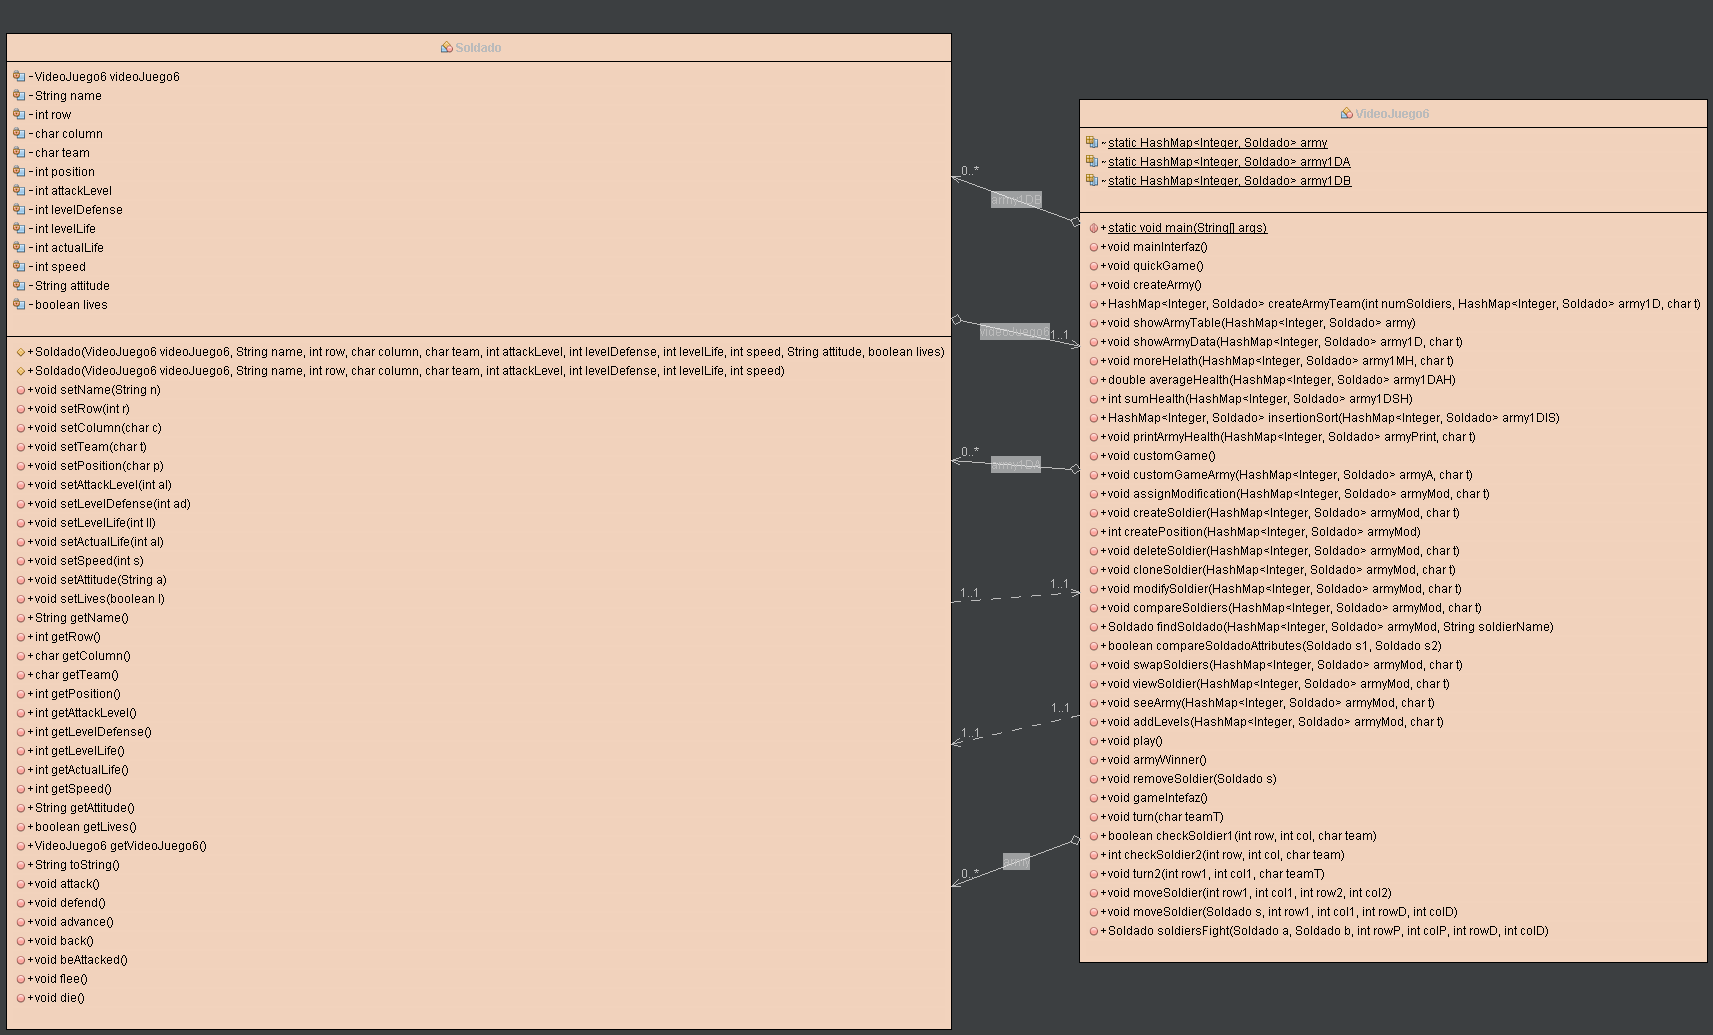
\includegraphics[width=1.1
    \textwidth,keepaspectratio]{img/12uml.png}
    \caption{}
\end{figure}

\href{https://github.com/hernanchoquehuanca/fp2-23b/blob/main/fase02/lab12/latex/img/12uml.png}{Diagrama 12 UML} para acceder al diagrama UML del repositorio y se observe con más claridad.

%------------------------------ ESTRUCTURA DE LABORATORIO --------------------------

\newpage

\subsection{Estructura de laboratorio 12} %%CAMBIAR NUMERO DE LAB
\begin{itemize}	
	\item El contenido que se entrega en este laboratorio es el siguiente:
\end{itemize}

%---------------------------------------- TREE -------------------------------------

\begin{lstlisting}[style=ascii-tree]

    lab12
    |   Soldado.java
    |   VideoJuego6.java
    |
    |───latex
        |   Informe_Lab12.pdf
        |   Informe_Lab12.tex
        |
        |───img
        |       12addLevels.png     
        |       12compareSoldiers.png  
        |       12customGame.png      
        |       12deleteSoldier.png  
        |       12swapSoldiers.png  
        |       12viewSoldier.png  
        |       logo_episunsa.png  
        |       mainInterfaz.png
        |       12cloneSoldier.png  
        |       12createSoldier.png    
        |       12customGameArmy.png  
        |       12modifySoldier.png  
        |       12uml.png           
        |       logo_abet.png      
        |       logo_unsa.jpg      
        |       showArmyTable.png
        |
        |───src
                Soldado.java
                VideoJuego6.java

\end{lstlisting}    

\section{\textcolor{red}{Rúbricas}}
	
\subsection{\textcolor{red}{Entregable Informe}}
	\begin{table}[H]
		\caption{Tipo de Informe}
		\setlength{\tabcolsep}{0.5em} % for the horizontal padding
		{\renewcommand{\arraystretch}{1.5} % for the vertical padding
		\begin{tabular}{|p{3cm}|p{12cm}|}
			\hline
			\multicolumn{2}{|c|}{\textbf{\textcolor{red}{Informe}}}  \\
			\hline 
			\textbf{\textcolor{red}{Latex}} & \textcolor{blue}{El informe está en formato PDF desde Latex,  con un formato limpio (buena presentación) y fácil de leer.}   \\ 
			\hline 
		\end{tabular}
	}
	\end{table}
	
\clearpage

%------------------------------ RÚBRICA DE EVALUACIÓN ------------------------------
 
\subsection{\textcolor{red}{Rúbrica para el contenido del Informe y demostración}}
\begin{itemize}			
	\item El alumno debe marcar o dejar en blanco en celdas de la columna \textbf{Checklist} si cumplió con el ítem correspondiente.
	\item Si un alumno supera la fecha de entrega,  su calificación será sobre la nota mínima aprobada, siempre y cuando cumpla con todos lo ítems.
	\item El alumno debe auto calificarse en la columna \textbf{Estudiante} de acuerdo a la siguiente tabla:
	
    \begin{table}[ht]
    	\caption{Niveles de desempeño}
    	\begin{center}
    		\begin{tabular}{ccccc}
        	\hline
        	& \multicolumn{4}{c}{Nivel}\\
        	\cline{1-5}
        	\textbf{Puntos} & Insatisfactorio 25\%& En Proceso 50\% & Satisfactorio 75\% & Sobresaliente 100\%\\
        	\textbf{2.0}&0.5&1.0&1.5&2.0\\
        	\textbf{4.0}&1.0&2.0&3.0&4.0\\
        	\hline
    		\end{tabular}
    	\end{center}
    \end{table}	
\end{itemize}

%------------------------------------ EVALUACIÓN -----------------------------------

\begin{table}[H]
    \caption{Rúbrica para contenido del Informe y demostración}
    \setlength{\tabcolsep}{0.5em} % for the horizontal padding
    {\renewcommand{\arraystretch}{1.5}% for the vertical padding
    %\begin{center}
    \begin{tabular}{|p{2.7cm}|p{7cm}|x{1.3cm}|p{1.2cm}|p{1.5cm}|p{1.1cm}|}
        \hline
        \multicolumn{2}{|c|}{Contenido y demostración} & Puntos & Checklist & Estudiante & Profesor\\
        \hline
        \textbf{1. GitHub} & Hay enlace URL activo del directorio para el  laboratorio hacia su repositorio GitHub con código fuente terminado y fácil de revisar. &2 &X &2 & \\ 
        \hline
        \textbf{2. Commits} &  Hay capturas de pantalla de los commits más importantes con sus explicaciones detalladas. (El profesor puede preguntar para refrendar calificación). &4 &X &4 & \\ 
        \hline 
        \textbf{3. Código fuente} &  Hay porciones de código fuente importantes con numeración y explicaciones detalladas de sus funciones. &2 &X &2 & \\ 
        \hline 
        \textbf{4. Ejecución} & Se incluyen ejecuciones/pruebas del código fuente  explicadas gradualmente. &2 &X &2 & \\ 
        \hline			
        \textbf{5. Pregunta} & Se responde con completitud a la pregunta formulada en la tarea.  (El profesor puede preguntar para refrendar calificación).  &2 &X &2 & \\ 
        \hline	
        \textbf{6. Fechas} & Las fechas de modificación del código fuente están dentro de los plazos de fecha de entrega establecidos. &2 &X &2 & \\ 
        \hline 
        \textbf{7. Ortografía} & El documento no muestra errores ortográficos. &2 &X &2 & \\ 
        \hline 
        \textbf{8. Madurez} & El Informe muestra de manera general una evolución de la madurez del código fuente,  explicaciones puntuales pero precisas y un acabado impecable.   (El profesor puede preguntar para refrendar calificación).  &4 &X &3 & \\ 
        \hline
        \multicolumn{2}{|c|}{\textbf{Total}} &20 & &19 & \\ 
        \hline
    \end{tabular}
    %\end{center}
    %\label{tab:multicol}
    }
\end{table}
\clearpage

%------------------------------ REFERENCIAS ------------------------------

\section{Referencias}
\begin{itemize}			
    \item \url{https://docs.oracle.com/javase/tutorial/java/nutsandbolts/variables.html}
    \item \url{https://docs.oracle.com/javase/8/docs/api/java/util/HashMap.html}
    \item \url{https://docs.oracle.com/javase/tutorial/java/javaOO/methods.html}
    \item \url{https://www.geeksforgeeks.org/insertion-sort/}
    \item \url{https://es.stackoverflow.com/questions/108171/}
\end{itemize}	
	
%\clearpage
%\bibliographystyle{apalike}
%\bibliographystyle{IEEEtranN}
%\bibliography{bibliography}
\end{document}